\documentclass[10 pt,usenames,dvipsnames, oneside]{article}
\usepackage{../../modelo-fracoes}
\graphicspath{{../../../Figuras/licao02/}}


\begin{document}

\begin{center}
  \begin{minipage}[l]{3cm}

\includegraphics[width=2cm]{../../../Figuras/logo}       
\end{minipage}\hfill
\begin{minipage}[r]{.8\textwidth}
 {\Large \scshape Atividade: Tortas repartidas em 8 fatias}  
\end{minipage}
\end{center}
\vspace{.2cm}

\ifdefined\prof
\begin{goals}
\begin{enumerate}

\item Compreender e usar a expressão ''$n$ oitavos de''{} como forma de identificar a quantidade equivalente a $n$ cópias de um oitavo da unidade, incluindo os casos em que $n$ é maior do que oito.
\item Reconhecer que uma mesma quantidade pode ser expressa por frações equivalentes de uma mesma unidade (por exemplo, ''meia torta''{} e ''quatro oitavos de torta'' representam a mesma quantidade de torta).

\end{enumerate}

\tcblower
\begin{multicols}{2}


\begin{itemize} %s
    \item Recomenda-se que a atividade seja desenvolvida em grupos de 3 a 5 alunos.
    \item As diversas soluções apresentadas pelos diferentes grupos devem ser discutidas com a turma inteira.
    \item É importante que a discussão conduza os alunos ao uso de oitavos:  ''quatro oitavos'', ''dez oitavos''{} e ''uma torta e dois oitavos''.
     \item As respostas esperadas para o Item c) podem surgir na resolução do Item b). Caso isso aconteça, recomenda-se que as frações corretas correspondentes a $4$ fatias de uma torta (metade de uma torta, dois quartos de uma torta, quatro oitavos de uma torta, etc.) sejam reconhecidas como tal, mas que, conforme solicitado pelo enunciado, a resposta deve ser dada em termos de oitavos.
     \item No Item c), é importante estimular o aluno a dar uma explicação para sua resposta: ''por que você pensou em metade de uma torta?''{}, ''Por que você pensou em dois quartos de uma torta?''{} etc. Espera-se que os alunos expressem que estas frações expressam a mesma quantidade da unidade torta. Não se pretende usar a nomenclatura ''frações equivalentes''.
\end{itemize}

\end{multicols}
\end{goals}




\bigskip
\begin{center}
{\Large \scshape Atividade}
\end{center}
\fi

Para a sobremesa do almoço de domingo, papai passou em uma confeitaria que vende tortas.
Cada torta está dividida em  igualmente em 8 fatias, como na figura abaixo.

\begin{center}
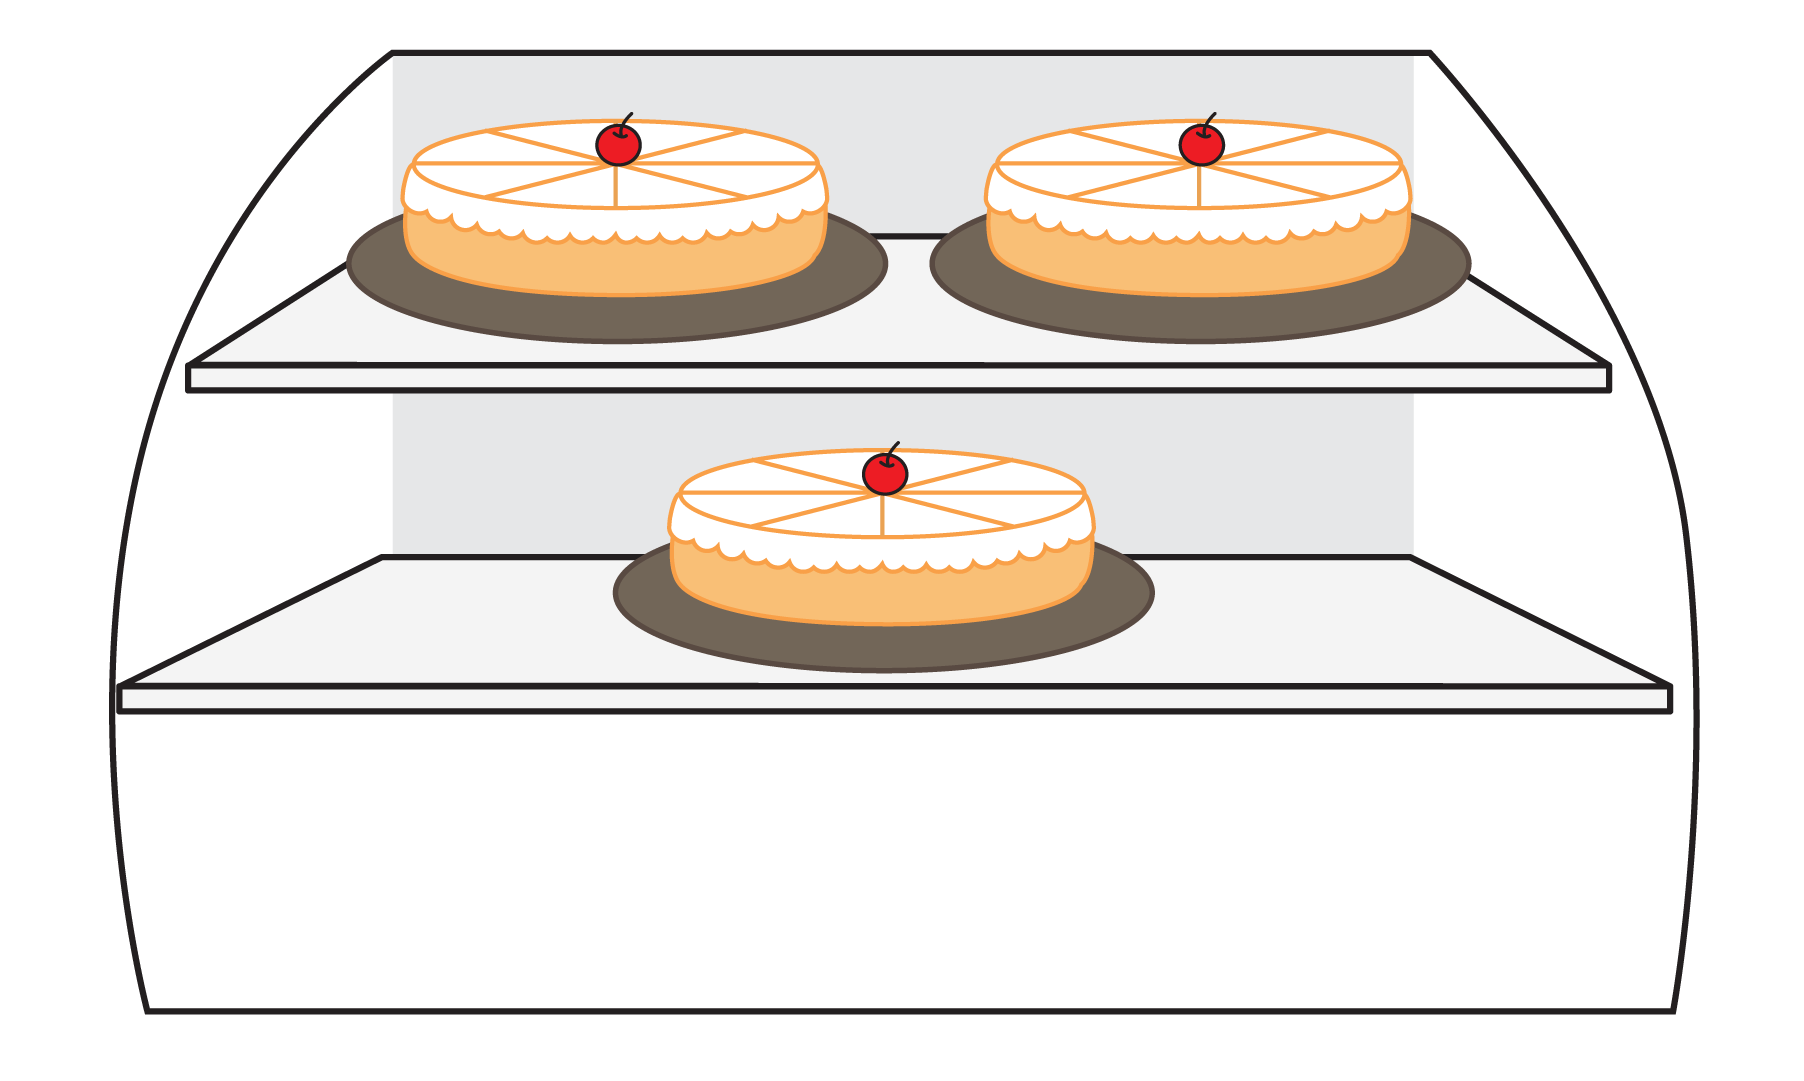
\includegraphics[width=.6\textwidth, keepaspectratio]{ativ3_fig01.png}
\end{center}

\begin{enumerate} [label=\alph*)] %s
  \item     Que fração de uma torta é uma fatia? Explique.
  \item     Domingo papai comprou 4 fatias, quantos oitavos de uma torta havia para a sobremesa?
  \item     Na pergunta anterior, apresente outra fração que represente a quantidade de torta que papai comprou. Explique sua resposta.
  \item     Hoje papai comprou 10 fatias de torta. Como podemos representar essa quantidade de torta em termos de frações de uma torta?
\end{enumerate} %s

\ifdefined\prof

\begin{solucao}

\begin{enumerate} [label=\alph*)] %s
    \item       Cada fatia é um oitavo de torta, pois cada torta está dividida em oito partes iguais.
    \item       Havia para a sobremesa quatro oitavos de torta.
    \item       Meia torta, pois quatro fatias de torta têm a mesma quantidade de torta que meia torta.

  \begin{center}
  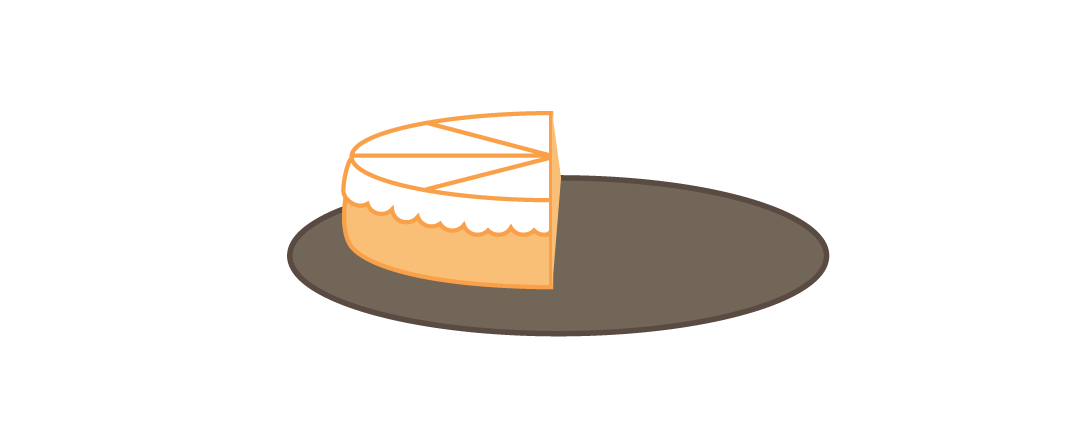
\includegraphics[width=175pt, keepaspectratio]{ativ3_resposta.png}
  \end{center}

    \item       Algumas respostas possíveis: dez oitavos de torta;  uma torta inteira e dois oitavos de torta; uma torta inteira e um quarto de torta.
\end{enumerate} %s

\end{solucao}
\fi

\end{document}